\documentclass[12pt]{article}

\usepackage[T1]{fontenc}
\usepackage{blindtext}
\usepackage[]{algorithm2e}
\usepackage{graphicx}
\usepackage{float}
\usepackage{amsfonts, amssymb, amsmath}
\usepackage[utf8]{inputenc}
\usepackage{xcolor}
\usepackage{booktabs} % For better table lines
\usepackage{appendix} % For appendices
\usepackage{hyperref}
\hypersetup{
    colorlinks=true,
    linkcolor=blue,
    filecolor=magenta,      
    urlcolor=blue,
    pdftitle={Overleaf Example},
    pdfpagemode=FullScreen,
    }

\parindent 0px

\graphicspath{ {../Results} }

\title{Comparativa de una Heurística con Fuerza Bruta para la solucion del problema TSP}
\author{Jesus Antonio Alpaca Rendon}
\date{\today}

\begin{document}

\maketitle

\section{Introducción}
El presente trabajo es una comparativa para la resolucion del problema
TSP (Traveling Salesman Problem) utilizando fuerza bruta contra una heuristica la cual
en teoria brinda resultados de manera mas optima.
El problema TSP es una problematica computacional la cual consta de hallar la mejor ruta que debe aplicar un viajero para visitar \textit{n} cantidad de ciudades solo una vez,
es decir, hallar el mejor camino Hamiltoniano. Para este informe se aplico un algoritmo de fuerza bruta, el cual consta de medir todos los pesos posibles del grafo, obteniendo el de menor costo.
Esto tiene una complejidad de \textit{n!} ya que a mas vertices, mayor cantidad de rutas por analizar.
Para el presente informe se utilizo graficos completos,es decir, todos sus nodos tienen el mismo grado y todos son conexos.
La heuristica que se decidio aplicar para el presente informe es la de ACO(Ant Colony Optimization), el cual es una heuristica
inspirada en el comportamiento de las hormigas que estan en colonia, enfocandonos en las rutas que toman para obtener comida y como van seleccionando la mejor ruta
considerando otros factores como las feromonas que dejan en el camino, tiempo de vaporizacion, etc.

\section{Heurística}
En esta sección, explora la heurística que estás utilizando y su relevancia para resolver el problema planteado.
La heuristica seleccionada para el presente trabajo es ACO(Ant Colony Optimization), esta heuristica como se menciono en la introduccion se inspira en el comportamiento
de las hormigas de colonia. Como se sabe, las hormigas salen de la colonia para buscar comida y traerla de vuelta, las hormigas para no perderse, dejan un rastro de feromonas
que les sirve de guia para poder regresar a la colonia. Sin embargo en un inicio no conocen el camino y es muy probable que tomen la ruta mas larga sin saberlo.
Con el tiempo las hormigas van generando diversos caminos dodne la feromona juega un papel muy importante en la desicion que deben tomar las hormigas,
ya que es un factor que podria definir mucho en la eleccion.Para la eleccion se tiene en cuenta las rutas que cumplen 2 requisitos:
\begin{itemize}
    \item Ruta mas corta.
    \item Ruta con mas cantidad de feromonas.
\end{itemize}
Conociendo este comportamiento, es como la heuristica de ACO nace e intenta emular este comportamiento, considerando esos 2 requisitos, siendo representados en un modelo matematico.

Para empezar debemos considerar no solo la matriz de adyancencia del grafo, sino tambien otra matriz que sera la matriz de feromonas, esta matriz sera una replica del grafo en cuanto
a vertices y caminos, sin embargo, los pesos seran distintos, ya que tendra un peso basado en la cantidad de feromonas que se depositen en el camino, por ejemplo hay especies de hormigas
que depositan mayor cantidad de feromonas cuando encuentran una fuente grande de comida. En este caso se dejara mayor cantidad de feromonas si encontramos un camino mas optimo y para ello
se utilizara el siguiente modelo matematico.

Calculo de la feromona: $$\Delta\tau_{i,j}^k={  \frac{1}{L_k}}$$

\textit{Delta Tau} representa la feromona que se colocara en la arista entre \textit{i,j}, siendo \textit{k} la cantidad de veces que pase la hormiga sobre esa ruta, siendo su valor 1/$L_k$

En caso la hormiga no vaya por ese camino, la feromona sera 0

Nosotros podemos realizar la suma para saber la cantidad de feromonas que tenemos en todo el camino:

$$\tau_{i,j}^k=\sum_{k=1}^{m} \Delta\tau_{i,j}^k$$

Algo que hay que tener muy en cuenta tambien, es la vaporizacion, ya que las feromonas no son para siempre, si bien el algoritmo tambien lo considera como un factor que puede obviarse,
como en el de la formula que la sumatoria seria correcta, sin embargo si queremos considerar la vaporizacion, la formular cambiaria de la siguiente forma para calcular su total:

$$\tau_{i,j}^k=\textcolor{red}{(1-\rho)\tau_{i,j}}+\sum_{k=1}^{m} \Delta\tau_{i,j}^k$$

Como podemos ver \textit{$\rho$} es una constante que hara el calculo de la vaporizacion,
su maximo nivel es 1 y su minimo nivel es 0 en caso no se quiera considerar. Como se menciono
es un valor opcional si se quiere emular correctamente el algoritmo lo mas parecido a una situacion real.


\vspace{25mm}

EJEMPLO

\vspace{5mm}

Tenemos un grafo completo de 4 vertices, la hormiga 1 pasa por todos los vertices una sola vez y costo total obtenido es de 14

$$L_1=14 \rightarrow \Delta\tau_{i,j}^1=\frac{1}{14}$$

Tenemos una segunda hormiga que va por otro camino y el costo total fue de 31

$$L_2=31 \rightarrow \Delta\tau_{i,j}^2=\frac{1}{31}$$

Recordemos que para ir calculando el total de feromonas dejadas por las hormigas es solo la suma. En una arista que solo paso la hormiga 1
, el total de feromonas dejadas sera de $\frac{1}{14}$, mientras que en una arista donde pasaron ambas, sera de $\frac{1}{14}+\frac{1}{31}$

En este ejemplo no estamos viendo la vaporizacion, digamos que lo colocamos al valor de \textit{$\rho$} el valor de 0.5, la sumatoria ahora seria asi:

$$0.5*1+\frac{1}{14}$$
$$0.5*1+\frac{1}{14}+\frac{1}{31}$$

De esta manera podemos ir armando nuestra matriz de feronomas a la par de nuestra matriz original.
Si bien esto es para la parte de como utilizar las feromonas, faltaria ver como es que se escoje el camino correcto.
El calculo de la probabilidad, justamente se da dependiendo de los datos que tenemos almacenados en nuestras matrices, tanto la matriz de adjacencia
como la de feromonas.
La formula es la siguiente:

$$P_{i,j}=\frac{(\tau_{i,j})(\eta_{i,j})}{\sum((\tau_{i,j})(\eta_{i,j}))}$$

Donde:\\

\hspace{1cm}$P_{i,j}$ es la probabilidad de escoger ese camino

\hspace{1cm}$\tau_{i,j}$ el valor de la feromona de esa arista

\hspace{1cm}$\eta_{i,j}$ el valor de: $\frac{1}{L_{i,j}}$ que es 1 sobre el costo real de la arista

\vspace{5mm}

Aquí nos daremos cuenta que es donde toma bastante importancia la feromona, ya que si la feromona es alta en un camino de costo alto, puede influir en tomar
desiciones distintas a las esperadas, son situaciones donde no sucedan a menudo debido a que siempre habra mayores probabilidades en caminos de costo bajo
llegando asi a la ruta mas optima posible y dependiendo de la cantidad de hormigas que pasen por ella dejando la feromona.

Un ultimo punto a considerar es, una vez que tenemos esa probabilidad aumentando y disminuyendo, como es que la manejamos en si ya que,
toda probabilidad va a ser utilizada para obtener un valor random, en este caso, es muy usual utilizar \textit{Roulette Wheel} como algoritmo de obtencion
de un valor de acuerdo a probailidades, en este caso Roulette Wheel, va generando una suma cumulativa de las propiedades, siendo el mayor numero 1 y el menor,
la menor probabilidad obtenida, a partir de ahi se genera un numero random y se analizar en cual de los intervalos de la suma es donde cae el numero random, veamos un ejemplo:

Imaginemos que seguimos con nuestro grafo completo de 4 vertices, la probabilidad para escoger la arista 1 es de 76\%, la arista 2 es de 19\% y por ultimo
la arista 3 del 5\%.

La suma cumulativa quedaria de esta forma:
\vspace{15mm}
$$\textit{r} = Random$$

$$Intervalo 1 = {0.24 < \textit{r} \leq 1 }$$

$$Intervalo 2 = {0.05 < \textit{r} \leq 0.24 }$$

$$Intervalo 3 = {0.00 \leq \textit{r} \leq 0.05 }$$

De esta manera, dependiendo el numero random que obtengamos, si cae en el intervalo 1,
ira a la arista 1, y asi con los demas posibles resultados.

De esta forma obtenemos el camino Hamiltoniano mas optimo segun esta heuristica.

\section{Implementación}
La implementacion de la heuristica y el algoritmo de fuerza bruta, fueron realizadas en C++ y los datos de testeo y otros
se encuentran en el siguiente link de Github:

- \href{https://github.com/Alpha004/AyEDJAAR2023/tree/main/Ejercicio_2}{Repositorio Jesus Alpaca Rendon Ejercicio 2} 

\section{Resultados}

Para tener la informacion clara, a continuacion se muestra las caracteristicas de la PC utilizada para la implementacion.

\begin{figure}[H]
\centering
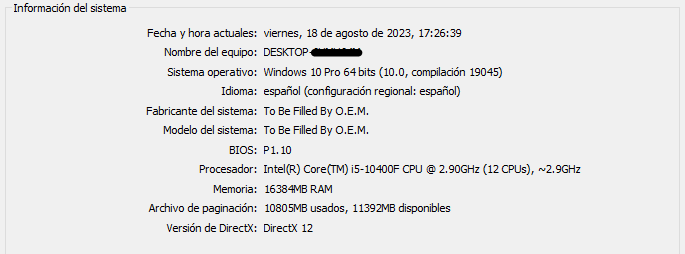
\includegraphics[width=\textwidth]{caracteristicas}
\caption{Caracteristicas del equipo PC utilizado}
\end{figure}

En este caso contaba con 16 gbs de ram lo cual permitio realizar pruebas a numeros mayores de vertices que se consideraron al inicio.
Se realizo pruebas con grafos completos de tamaños entre 4 - 14 vertices, puesto que al ejecutar la implementacion de Brute Force 
en un tamaño de 15, el programa tomaba mas de 2 horas sin dar resultado. Se estima que hubiera demorado entre 3 hoars y media y 4 horas
por cada iteracion.

Se ejecutaron 5 ejecuciones con el mismo tamaño de vertices para obtener un promedio de resultados aceptable.

A continuacion se muestra la grafica de resultados de la comparativa entre ACO y Brute Force para grafos completos.
Como podemos observar en la siguiente grafica de los resultados, la meta-heuristica ACO mantuvo un margen de tiempo similar en
diferentes cantidades de vertices para hallar la solucion mas optima, llegando incluso a grafos de 100 resultados con un tiempo aceptable. Sin embargo
no fueron considerados en la grafica de resultados actual debido a que Brute Force tomaba mucho tiempo a partir de los 15 vertices.

Un punto importante es que se considero utilizar 10 hormigas y 10 iteraciones para el algoritmo ACO, ya que con numeros menores, en este caso para los tamaños de 
vertices que se utilizaron, no habia mucho problema , pero numeros mayores como mas de 100 vertices, se recomienda utilizar un numero similar de hormigas para obtener
resultados mas precisos, por eso se decidio realizar 10 iteraciones siempre con 10 hormigas, ya que a partir de 3 o 4 hormigas siempre daba el mismo resultado


\begin{figure}[H]
\centering
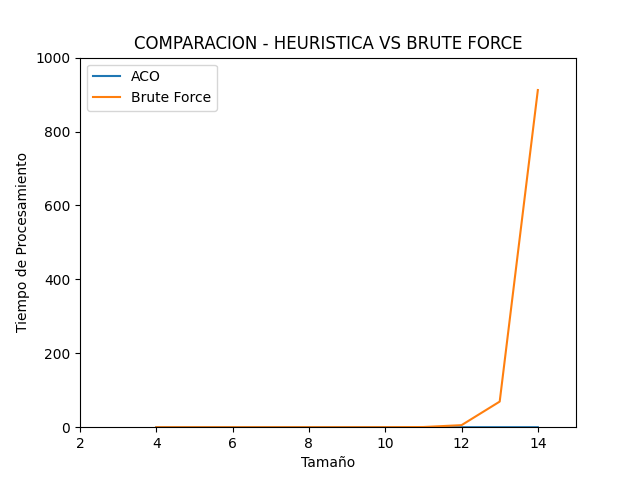
\includegraphics[width=\textwidth]{heuristica_results}
\caption{Grafica de Resultados}
\end{figure}

\section{Conclusiones}
Como conclusiones se puede indicar lo siguiente:

\begin{itemize}
    \item La meta-heuristica ACO logra definir la ruta mas optima en menos tiempo que Brute Force, logrando un punto de inflexion notorio
        desde que se brinda un grafo completo de grado 12, donde la grafica se desvia de una forma abrupta por el lado de Brute Force que tiene una complejidad de n! lo cual es bastante
    \item Las heuristicas brindan formas de resolver problemas de forma mas optima que las convencionales, siendo su importancia demostrada en la presente investigacion
\end{itemize}

\begin{thebibliography}{9}
    \bibitem{libro1}
    Blum, Christian. \textit{Ant colony optimization: Introduction and recent trends}. ELSEVIER, 2005.

    \bibitem{sitioweb1}
    Introduction to Ant Colony Optimization. URL: \texttt{https://www.javatpoint.com/introduction-to-ant-colony-optimization}
    
    \bibitem{sitioweb2}
    Professor Seyedali Mirjalili (Ali) - Ant Colony Optimization. URL: \texttt{https://seyedalimirjalili.com/aco}

\end{thebibliography}

% Appendices start here
\begin{appendices}

\section{Additional Information}
ANEXOS

\subsection{Datos de los Resultados}
A continuacion se anexan las tablas de los resultados obtenidos por las pruebas

\begin{table}[!ht]
    \centering
    \caption{Brute Force - Datos recopilados en segundos}
    \begin{tabular}{|l|l|l|l|l|l|l|}
    \hline
        DATA SIZE/ ITERATION & 1 & 2 & 3 & 4 & 5 & PROMEDIO \\ \hline
        4 & 0.001 & 0 & 0.002 & 0.001 & 0.001 & 0.001 \\ \hline
        5 & 0.001 & 0 & 0.001 & 0.001 & 0 & 0.0006 \\ \hline
        6 & 0 & 0.001 & 0.001 & 0 & 0.001 & 0.0006 \\ \hline
        7 & 0.001 & 0.001 & 0 & 0 & 0.001 & 0.0006 \\ \hline
        8 & 0.001 & 0.001 & 0.001 & 0.002 & 0.001 & 0.0012 \\ \hline
        9 & 0.006 & 0.005 & 0.006 & 0.006 & 0.006 & 0.0058 \\ \hline
        10 & 0.049 & 0.069 & 0.047 & 0.047 & 0.045 & 0.0514 \\ \hline
        11 & 0.477 & 0.51 & 0.478 & 0.477 & 0.477 & 0.4838 \\ \hline
        12 & 5.525 & 5.511 & 5.603 & 5.527 & 5.524 & 5.538 \\ \hline
        13 & 71.518 & 67.904 & 67.902 & 68.891 & 70.281 & 69.2992 \\ \hline
        14 & 916.421 & 914.371 & 956.838 & 891.3569 & 882.214 & 912.24018 \\ \hline
    \end{tabular}
\end{table}


\begin{table}[!ht]
    \centering
    \caption{Ant Colony Optimization - Datos recopilados en segundos}
    \begin{tabular}{|l|l|l|l|l|l|l|}
    \hline
        DATA SIZE/ ITERATION & 1 & 2 & 3 & 4 & 5 & PROMEDIO \\ \hline
        4 & 0 & 0.001 & 0 & 0.001 & 0.001 & 0.0006 \\ \hline
        5 & 0.001 & 0.001 & 0 & 0.001 & 0 & 0.0006 \\ \hline
        6 & 0.001 & 0.001 & 0.001 & 0.001 & 0.001 & 0.001 \\ \hline
        7 & 0.001 & 0.002 & 0.001 & 0.002 & 0.002 & 0.0016 \\ \hline
        8 & 0.003 & 0.003 & 0.003 & 0.002 & 0.002 & 0.0026 \\ \hline
        9 & 0.004 & 0.003 & 0.004 & 0.004 & 0.004 & 0.0038 \\ \hline
        10 & 0.005 & 0.005 & 0.005 & 0.005 & 0.005 & 0.005 \\ \hline
        11 & 0.007 & 0.006 & 0.007 & 0.007 & 0.007 & 0.0068 \\ \hline
        12 & 0.008 & 0.009 & 0.009 & 0.009 & 0.009 & 0.0088 \\ \hline
        13 & 0.011 & 0.012 & 0.011 & 0.011 & 0.011 & 0.0112 \\ \hline
        14 & 0.014 & 0.014 & 0.013 & 0.014 & 0.014 & 0.0138 \\ \hline
    \end{tabular}
\end{table}

\end{appendices}
\end{document}
